\documentclass[10pt]{article}
\usepackage[a4paper,margin=1in]{geometry}
\usepackage[T1]{fontenc}
\usepackage{newtxtext,newtxmath}
\usepackage{microtype}
\usepackage{amsmath}
\usepackage{booktabs}
\usepackage{graphicx}
\usepackage{xcolor}
\usepackage{caption}
\usepackage{tikz}
\usetikzlibrary{arrows.meta,positioning,fit,calc}
\usepackage[numbers,sort&compress]{natbib}
\usepackage[colorlinks=true,linkcolor=blue!50!black,citecolor=blue!50!black,urlcolor=blue!50!black]{hyperref}
\usepackage[section]{placeins}
\usepackage{algorithm}
\usepackage{algpseudocode}

\newcommand{\pend}[1]{\textcolor{red}{#1}}  % numbers still to be filled in from pending runs
\newcommand{\RT}[1]{\mathrm{RT}_{#1}}
\makeatletter\newcommand{\tabinput}[1]{\@@input #1 }\makeatother  % \input is not expandable inside tabular
\captionsetup{font=small,labelfont=bf}

\title{Round-Trip Refinement:\\A Training-Free Sampler for Next-Concept Language Models}
\author{Pierre Khoury\\{\small MSc Advanced Computing, King's College London}\\{\small\texttt{pierrecurrency@gmail.com}}}
\date{}

\begin{document}
\maketitle

\begin{abstract}
Next-Concept Modeling (NCM) generates text coarse to fine: a multiscale residual VQ-VAE turns a sequence into twelve levels of discrete codes, and a transformer predicts one whole level per pass, so a 128-token sequence takes eleven generator passes. We find that the code stacks NCM samples are not the stacks its own tokenizer would assign to the text they decode to: re-encoding a generated sample rewrites 61--96\% of the codes at each of the six coarsest levels, yet the re-encoded stack decodes back to the same text for 98\% of samples. We propose \emph{round-trip refinement}, a training-free sampler: decode the draft, re-encode the text with the tokenizer, keep the re-encoded coarse levels, and regenerate the fine levels with the unchanged generator. On the released TinyStories and LM1B checkpoints, using the authors' own sampling and evaluation code, one round lowers GPT-2 Large generative perplexity by 17\% on TinyStories and 22\% on LM1B (large) at equal unigram entropy, for six extra generator passes; two or three rounds reach $-31\%$ and $-29\%$. Resampling the fine levels without re-encoding gives no gain, and re-quantizing the final latent instead of the text, a latent-space analogue of image scale-travel, recovers at most half of it. The gain is not a temperature effect in disguise: at matched corpus diversity refinement sits 10--15\% below the temperature frontier at the released temperature, where an exact 11-pass twin without the round trip gains nothing, and it does not sharpen real human text. Combined with a per-level temperature schedule (hot coarse levels, cool fine levels), which on its own already moves the TinyStories frontier by up to 21\%, refinement adds a further 4--10 points; the resulting samplers are about 21\% more fluent than the released one at equal or higher diversity on held-out seeds of TinyStories and LM1B. All findings replicate on held-out seeds and across three LM1B model sizes, with gains that do not shrink with size; an LLM judge prefers refined stories to the released sampler's (0.63), and MAUVE against human text rises from 0.88 to 0.94--0.96. On Sudoku-hard, refinement solves 14--19 more of 1{,}000 puzzles while breaking at most one, but it does not help on easier puzzles, and with an exact verifier plain resampling is the better use of extra compute. On XSum, refined summaries are 16\% more fluent with a small ROUGE gain; on WMT14, whose tokenizer round trip is lossy, refinement does not help. The image next-scale model VAR also samples non-canonical code stacks, but there the round trip through pixels does not improve FID. We also report what did not work on this budget: early exit, level skipping, level-dropout training, joint tokenizer--generator fine-tuning, training on the model's own errors, and distilling the refined sampler back into the generator, which matches the released perplexity only by giving up diversity. Code is available at \url{https://github.com/PierreKhoury1/ncm-round-trip}.
\end{abstract}

\section{Introduction}

Diffusion language models generate in parallel but need many denoising steps, each over the full sequence \citep{sahoo2024mdlm,wang2025remdm}. Next-Concept Modeling \citep[NCM;][]{kumbong2026ncm} takes a different route, borrowed from next-scale prediction in vision \citep{tian2024var,kumbong2025hmar}: a multiscale residual VQ-VAE encodes a 128-token sequence into $K{=}12$ levels of codes, from one code for the whole sequence to 128 codes at the finest level, and a transformer generates the levels coarse to fine, all codes of a level in parallel. NCM reaches the generative perplexity of strong diffusion baselines with an order of magnitude fewer function evaluations (NFE).

Each NCM level is sampled conditioned on the generator's own samples of the coarser levels. In training, by contrast, the coarser levels are the tokenizer's codes for real text, perturbed by uniform code replacement \citep[``conditioning corruption'';][\S3.4]{kumbong2026ncm}. Residual quantization is many-to-one: many code stacks decode to the same tokens, and the tokenizer always produces one particular stack, the greedy residual quantization of its encoder output. A sampled stack need not be that one. We measure this directly: decoding a generated sample and re-encoding the text changes 61--96\% of the codes at each of the six coarsest levels (20--72\% at the finer ones), yet decoding the re-encoded stack gives back exactly the same text for 98\% of samples (Section~\ref{sec:why}).

This suggests a simple repair. Once a draft exists, the tokenizer can tell us how \emph{it} would have encoded that text. We keep the re-encoded coarse levels, which now form a stack of the kind the generator saw in training, and let the generator redo the fine levels on top of them (Figure~\ref{fig:method}). The procedure needs no training, no new parameters and no change to the authors' sampler or decoder; it reuses the released generator, tokenizer and evaluation scripts as they are.

\paragraph{Contributions.}
\begin{itemize}
\item A diagnosis: NCM's sampled code stacks are non-canonical (not the stacks the tokenizer assigns to their own decoded text), and re-encoding replaces them by canonical ones without changing the text (Section~\ref{sec:why}).
\item Round-trip refinement, a training-free sampler with one knob, the restart level $k$ (Section~\ref{sec:method}), and ablations showing that the re-encoding through text, not the extra passes, carries the gain.
\item An evaluation on nine released checkpoints under the authors' protocols, with the temperature frontier, three diversity measures and exact 11-pass temperature twins as controls (Section~\ref{sec:results}): $-17\%$ to $-31\%$ gen-PPL on TinyStories and $-22\%$ to $-29\%$ on LM1B large, 10--15\% beyond the temperature frontier, and clear failure cases (translation with a lossy tokenizer, easy Sudoku).
\item Evidence beyond Gen.\ PPL: held-out seeds, an LLM judge, MAUVE against human text, a trend over three model sizes, and a reasoning task (Sudoku) where refinement fixes puzzles without breaking solved ones (Sections~\ref{sec:heldout}--\ref{sec:sudoku}).
\item Negative results for six training-side ideas, including the two the NCM paper lists as future work, so that others need not repeat them (Section~\ref{sec:negative}).
\end{itemize}

\begin{figure}[!htb]
\centering
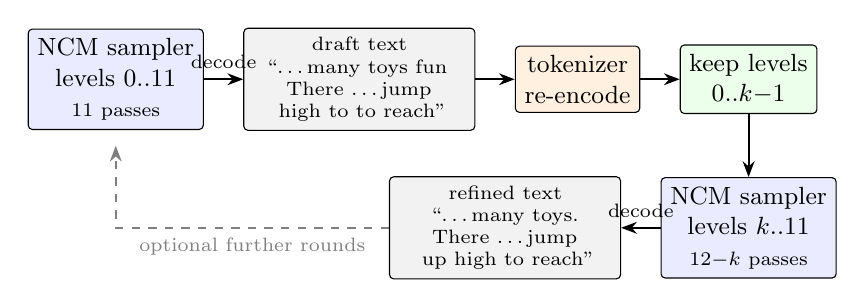
\begin{tikzpicture}[
  node distance=4mm and 5mm,
  box/.style={draw, rounded corners=1.5pt, minimum height=7mm, align=center, font=\small},
  gen/.style={box, fill=blue!8},
  tok/.style={box, fill=orange!12},
  txt/.style={box, fill=gray!10, text width=27mm, font=\scriptsize},
  arr/.style={-{Stealth[length=2mm]}, thick}]
\node[gen] (draft) {NCM sampler\\levels $0..11$\\\scriptsize 11 passes};
\node[txt, right=of draft] (t1) {draft text\\``\dots many toys fun There \dots jump high to to reach''};
\node[tok, right=of t1] (enc) {tokenizer\\re-encode};
\node[box, right=of enc, fill=green!8] (keep) {keep levels\\$0..k{-}1$};
\node[gen, below=8mm of keep] (regen) {NCM sampler\\levels $k..11$\\\scriptsize $12{-}k$ passes};
\node[txt, left=of regen] (t2) {refined text\\``\dots many toys. There \dots jump up high to reach''};
\draw[arr] (draft) -- node[above,font=\scriptsize]{decode} (t1);
\draw[arr] (t1) -- (enc);
\draw[arr] (enc) -- (keep);
\draw[arr] (keep) -- (regen);
\draw[arr] (regen) -- node[above,font=\scriptsize]{decode} (t2);
\draw[arr, dashed, gray] (t2.west) -| node[pos=0.25,below,font=\scriptsize]{optional further rounds} ($(draft.south)+(0,-2mm)$);
\end{tikzpicture}
\caption{Round-trip refinement ($\RT{k}$). The draft is decoded to text and re-encoded by the tokenizer; the re-encoded coarse levels replace the sampled ones and the generator regenerates levels $k..11$. The text is a real example (TinyStories, seed 1, sample 4; full text in Appendix~\ref{app:samples}).}
\label{fig:method}
\end{figure}

\section{Background: Next-Concept Modeling}
\label{sec:background}

\paragraph{Tokenizer.} An encoder $E$ maps a token sequence $x \in \mathcal{V}^{L}$ ($L{=}128$) to features $z \in \mathbb{R}^{L\times d}$. A multiscale residual quantizer with level lengths $\ell_0,\dots,\ell_{K-1}$ (for TinyStories $1,8,16,24,32,40,52,64,76,92,108,128$) then picks codes greedily,
\begin{equation}
r_k = \arg\min_{j} \big\| \mathrm{Down}_{\ell_k}(z - \hat z_{k-1}) - e_{k,j} \big\|, \qquad \hat z_k = \hat z_{k-1} + \phi_k\!\big(\mathrm{Up}_L(e_{k,r_k})\big),
\label{eq:rq}
\end{equation}
with codebooks $e_k$ of 4{,}096 entries and $\hat z_{-1}{=}0$. A decoder $D$ maps $\hat z_{K-1}$ back to token logits. We write $Q(E(x))$ for the full code stack of $x$ and $\mathrm{dec}(r)$ for decoding a stack to tokens with the authors' token picker (argmax, with frequency and adjacency penalties on LM1B).

\paragraph{Generator.} The NCM transformer predicts all $\ell_k$ codes of level $k$ in one pass from the reconstruction $\hat z_{k-1}$ resized to $\ell_k$ positions, with block-diagonal attention so that pass $k$ processes only $\ell_k$ positions. Unconditional generation draws $r_0$ from a unigram prior and then runs $K{-}1{=}11$ passes. Training uses teacher forcing on $Q(E(x))$ for real text, with a share of the input codes replaced uniformly at random (mean rate 0.5, decreasing with level), while targets stay clean.

\section{Round-Trip Refinement}
\label{sec:method}

\begin{algorithm}[t]
\caption{Round-trip refinement with restart levels $k_1, \dots, k_m$}
\label{alg:rt}
\begin{algorithmic}[1]
\State $r \gets \textsc{NCM-Sample}()$ \Comment{draft: $r_0$ from the prior, then $K{-}1$ passes}
\State $x \gets \mathrm{dec}(r)$
\For{$k \in (k_1, \dots, k_m)$}
  \State $r' \gets Q(E(x))$ \Comment{re-encode the current text}
  \State $r \gets \textsc{NCM-Sample}(\text{levels } 0..k{-}1 \text{ fixed to } r'_{0..k-1})$ \Comment{$K{-}k$ passes}
  \State $x \gets \mathrm{dec}(r)$
\EndFor
\State \Return $x$
\end{algorithmic}
\end{algorithm}

Algorithm~\ref{alg:rt} gives the sampler. One round with restart level $k$, written $\RT{k}$, costs $K{-}k$ extra generator passes plus one tokenizer encoder pass. Multiple rounds are written $\RT{5}{\times}2$ (two rounds from level 5) or $\RT{3}{+}\RT{6}{+}\RT{9}$ (three rounds from successively finer levels). Because pass $k$ processes $\ell_k$ positions, regenerating levels $6..11$ re-processes 520 of the 640 positions of a full sample; FLOPs therefore grow by about $1.8\times$ for $\RT{6}$ and $3.3\times$ for three rounds, somewhat more than the NFE ratios of $1.5\times$ and $2.6\times$ suggest.

\paragraph{Implementation.} We do not reimplement sampling. The authors' \texttt{generate} calls a per-level sampling function once per level; we wrap that function so that, for levels below $k$, it returns the re-encoded codes instead of sampling (Appendix~\ref{app:impl}). Code embeddings, level encodings, heads, attention masks and the token picker are therefore exactly the released ones. As a check, forcing \emph{every} level to the re-encoded stack reproduces the draft text exactly on TinyStories (8/8 samples tested), 27/32 on XSum and only 15/32 on WMT14, whose tokenizer round trip is lossy (Section~\ref{sec:cond}).

\paragraph{Ablations.} Two controls isolate where the gain comes from. \emph{Resample}$_k$ keeps the draft's own codes for levels below $k$ and regenerates the rest; it costs the same as $\RT{k}$ but involves no re-encoding, so it draws the fine levels from the same conditional distribution as the draft did. \emph{LatentRQ}$_k$ re-quantizes the draft's latent $\hat z_{K-1}$ with Eq.~\eqref{eq:rq} instead of decoding and re-encoding the text; it is the text analogue of scale-travel in DiverseVAR \citep{park2025diversevar}.

\section{Experimental setup}
\label{sec:setup}

\paragraph{Checkpoints and sampling.} We use the released NCM checkpoints for TinyStories \citep{eldan2023tinystories} (88.6M generator), LM1B \citep{chelba2013lm1b} small and large, XSum \citep{narayan2018xsum} and WMT14 de--en \citep{bojar2014wmt}, with the released evaluation configurations: temperature 1, no top-$k$/top-$p$ and no guidance for TinyStories and LM1B (LM1B with the configured frequency and adjacency penalties in the token picker), greedy decoding for XSum and WMT14. Refinement rounds use the same settings as the draft unless stated otherwise.

\paragraph{Metrics.} For TinyStories we report generative perplexity (Gen.\ PPL) under GPT-2 Large \citep{radford2019gpt2} and the mean per-sample unigram entropy $H$ of GPT-2 tokens, as in the NCM paper; for LM1B we use the authors' FLM protocol (corpus perplexity over the first 128 GPT-2 tokens of the decoded ids, entropy over raw ids). Because Gen.\ PPL can be lowered by reducing diversity \citep{pynadath2026frontiers,franca2026hacking}, we add corpus distinct-3 (unique word trigrams over all trigrams), cross-sample 4-gram overlap (xs-4, share of a sample's 4-grams that occur in another sample; lower is more diverse), and the rate of adjacent doubled words, and we compare every sampler with the \emph{temperature frontier}: the released sampler at $\tau \in \{1, 0.95, 0.9, 0.85, 0.8, 0.7\}$, interpolated at the same distinct-3 (TinyStories) or entropy (LM1B). XSum is scored with ROUGE-1/2/L \citep{lin2004rouge} plus GPT-2 Gen.\ PPL of the summaries, WMT14 with sacreBLEU \citep{post2018sacrebleu} and chrF. Unconditional results average three seeds of 256 samples each. All samplers of a seed share their level-0 draws; drafts are identical across samplers only for the first batch of each seed (samples 0--127 on TinyStories, 0--31 on LM1B), because refinement rounds consume random numbers before the second batch. Conditional results use the first 1{,}000 test documents.

\paragraph{Reproduction.} Our pipeline gives $16.15 \pm 0.17$ Gen.\ PPL for the released TinyStories sampler (seeds 1--3) and $16.32$ on seeds 4--6; the closest number in the NCM paper is 15.41, from its block-diagonal attention ablation, which is not the released evaluation run. All comparisons below are against our own reproduction, under identical code and seeds.

\section{Results}
\label{sec:results}

\subsection{TinyStories}

\begin{table}[!htb]
\centering
\small
\setlength{\tabcolsep}{4pt}
\begin{tabular}{lrrrrrrrr}
\toprule
Sampler & NFE & Gen.\ PPL $\downarrow$ & $\Delta$ & $H$ & dist-3 $\uparrow$ & xs-4 $\downarrow$ & dup\% $\downarrow$ & vs.\ $\tau$ frontier \\
\midrule
\tabinput{tables/ts.tex}
\bottomrule
\end{tabular}
\caption{TinyStories, released checkpoint, GPT-2 Large, 3 seeds $\times$ 256 samples (mean $\pm$ s.d.\ over seeds). $\Delta$: change in Gen.\ PPL against the released sampler. Last column: Gen.\ PPL relative to the temperature curve ($\tau{=}0.7..1.2$) interpolated at the same corpus distinct-3, per seed then averaged (negative = better than changing the temperature). Every refinement variant beats the released sampler on all three seeds.}
\label{tab:ts}
\end{table}

\begin{figure}[!htb]
\centering
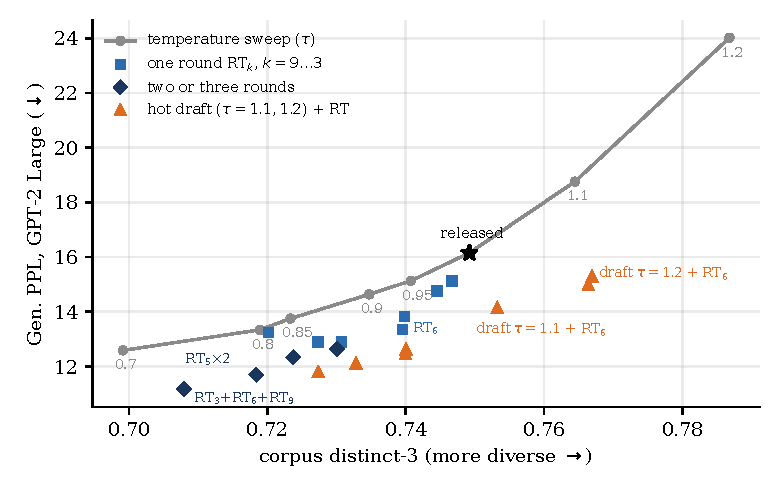
\includegraphics[width=0.72\linewidth]{figs/ts_frontier.pdf}
\caption{TinyStories: Gen.\ PPL against corpus distinct-3. Lowering the temperature buys fluency with diversity along the grey curve; round-trip refinement lands below it at every restart level, and further rounds move along a lower curve.}
\label{fig:tsfrontier}
\end{figure}

Table~\ref{tab:ts} and Figure~\ref{fig:tsfrontier} give the main result. One round from level 6 lowers Gen.\ PPL from 16.15 to 13.36 ($-17.3\%$, all seeds) with unigram entropy essentially unchanged (3.974 vs.\ 3.980). Restarting from coarser levels helps up to $k{=}4$--$5$ ($-20\%$); restarting from level 3 rewrites too much of the content and the gain shrinks. More rounds keep improving: $\RT{5}{\times}2$ reaches 11.70 ($-27.6\%$) and $\RT{3}{+}\RT{6}{+}\RT{9}$ reaches 11.17 ($-30.9\%$), closing 65\% of the gap to human text (8.51).

\paragraph{Not a temperature effect.} Lower temperature also lowers Gen.\ PPL: $\tau{=}0.8$ gives 13.34, the same as $\RT{6}$. But it does so by giving up diversity, to distinct-3 0.719 and cross-sample overlap 0.191, where $\RT{6}$ keeps 0.740 and 0.170. Interpolating the temperature curve ($\tau$ from 0.7 to 1.2) at each sampler's own distinct-3, single rounds are 6--12\% better than temperature for $k{=}5..8$ and multiple rounds 10--14\% better; sampling levels 6--11 at $\tau{=}0.8$ ($\tau_{\geq 6}{=}0.8$, in the draft and in the round) gives the largest single-round margin, $-14.4\%$. Refinement also removes errors that temperature does not touch: adjacent doubled words (``to to'', ``quickly quickly''), a typical failure of predicting a whole level in parallel, fall from 0.39\% of words to 0.23\% under $\RT{6}$, while every temperature setting leaves them at 0.32--0.36\%.

\begin{figure}[!htb]
\centering
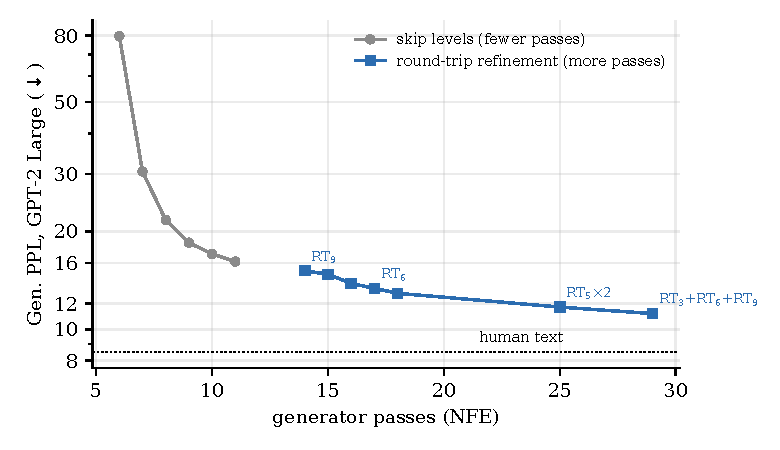
\includegraphics[width=0.66\linewidth]{figs/ts_nfe.pdf}
\caption{Quality against generator passes on TinyStories (GPT-2 Large). Grey: the released generator with middle levels skipped (fewer passes), which degrades quickly. Blue: round-trip refinement, which turns extra passes into steady gains. Dotted: human-written validation openings.}
\label{fig:nfe}
\end{figure}

\paragraph{Compute.} Figure~\ref{fig:nfe} places refinement on a quality--compute curve. Skipping levels of the released sampler to save passes costs $+6\%$ for one pass and $+89\%$ for four; refinement spends 3--18 extra passes for $-6\%$ to $-31\%$. NCM's speed advantage over diffusion LMs is 10--31$\times$ in wall-clock \citep{kumbong2026ncm}, so even the three-round sampler (29 passes, about $3.3\times$ the FLOPs) stays far cheaper than the 128--1{,}024-step diffusion samplers NCM is compared with.

\subsection{LM1B}

\begin{table}[!htb]
\centering
\small
\setlength{\tabcolsep}{4pt}
\begin{tabular}{lrrrrrrr}
\toprule
Sampler & NFE & Gen.\ PPL $\downarrow$ & $\Delta$ & $H$ & dist-3 $\uparrow$ & xs-4 $\downarrow$ & seeds better \\
\midrule
\tabinput{tables/lm1b.tex}
\bottomrule
\end{tabular}
\caption{LM1B, released small and large checkpoints, authors' FLM protocol (GPT-2 Large), 3 seeds $\times$ 256 samples. Diversity measured on BERT word-piece ids. Refinement improves Gen.\ PPL at equal or higher entropy; temperature cannot.}
\label{tab:lm1b}
\end{table}

\begin{figure}[!htb]
\centering
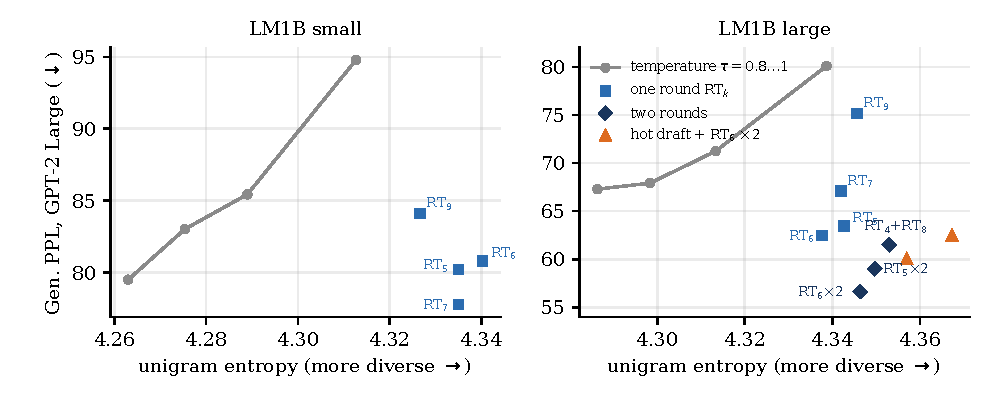
\includegraphics[width=0.92\linewidth]{figs/lm1b_frontier.pdf}
\caption{LM1B: Gen.\ PPL against unigram entropy. Temperature (grey) trades entropy for perplexity; refinement moves straight down, and on the large model two rounds reach $-29\%$ at slightly \emph{higher} entropy.}
\label{fig:lm1b}
\end{figure}

The result carries over to LM1B, a different domain (news sentences), tokenizer (BERT word pieces) and evaluation protocol (Table~\ref{tab:lm1b}, Figure~\ref{fig:lm1b}). On the small model one round lowers Gen.\ PPL by 11--18\%, on the large model by 6--22\%, on every seed and at equal or higher entropy, whereas $\tau{=}0.8$ reaches $-16\%$ only by dropping entropy from 4.339 to 4.286. Two rounds from level 6 reach 56.63 on the large model ($-29.3\%$) at entropy 4.346. The released medium model behaves the same way ($\RT{6}$ $-20.6\%$, $\RT{6}{\times}2$ $-28.8\%$ at entropy 4.342 vs.\ 4.339), and the gain of $\RT{6}$ does not shrink with model size: $-14.8\%$ (small), $-20.6\%$ (medium), $-22.0\%$ (large), which suggests the effect is not an artefact of a weak generator. Entropy is the least sensitive diversity axis on LM1B; measured on distinct-3 of the raw ids, $\RT{6}$ is 13--17\% and $\RT{6}{\times}2$ 17--21\% below the temperature curve on every seed (1--6), and the hot-draft sampler of Section~\ref{sec:hot} reaches $-21\%$ at the released sampler's distinct-3 (0.894 vs.\ 0.896).

\subsection{Conditional generation}
\label{sec:cond}

\begin{table}[!htb]
\centering
\small
\begin{tabular}{llrrrrr}
\toprule
Task & Sampler & NFE & R-1 & R-2 & R-L & Gen.\ PPL \\
\midrule
\tabinput{tables/cond.tex}
\bottomrule
\end{tabular}
\caption{Conditional tasks, released checkpoints, greedy decoding as configured, 1{,}000 test documents. XSum: refinement makes summaries more fluent with a small ROUGE gain; two rounds hurt. WMT14 de--en: refinement lowers BLEU, because the tokenizer round trip itself changes the output.}
\label{tab:cond}
\end{table}

On XSum (Table~\ref{tab:cond}), one round from level 3 raises ROUGE-1/2/L by $+0.25/+0.25/+0.33$ and lowers the Gen.\ PPL of the summaries from 82.4 to 69.5 ($-16\%$); two rounds overshoot. On WMT14 refinement lowers BLEU at every restart level, least for the coarsest restart ($\RT{4}$: 20.45 vs.\ 20.51) and by over 4 points for $\RT{6}$. The sanity check of Section~\ref{sec:method} explains why: re-encoding a WMT14 output and decoding it again, with no regeneration at all, already changes 17 of 32 outputs. When the tokenizer cannot reproduce its own outputs, the round trip injects errors, and in translation exact wording is what the metric rewards. Round-trip refinement therefore needs a tokenizer whose round trip is (near-)lossless on generated text; on TinyStories it is exact.

\subsection{Why the round trip helps}
\label{sec:why}

\paragraph{Sampled stacks are non-canonical.} Figure~\ref{fig:changed} shows, for 768 TinyStories drafts, the share of codes per level that change when the draft's stack is replaced by the tokenizer's stack for its decoded text: 96\% of the single level-0 codes, 61--84\% at levels 1--5, and 20--72\% at the finer levels. Yet decoding the re-encoded stack reproduces 751 of the 768 drafts exactly (97.8\%, and 99.98\% of tokens). The generator's stack and the tokenizer's stack are two different descriptions of the same text, and only the second is the kind of stack the generator conditions on in training, where its inputs are tokenizer stacks with uniform noise.

\paragraph{The re-encoding is what helps.} Table~\ref{tab:ablation} separates the ingredients. Regenerating levels 6--11 conditioned on the draft's own coarse codes (Resample$_6$) costs the same six passes as $\RT{6}$ but gives no gain at all (16.43 vs.\ 16.15 on TinyStories, $+0.6\%$ on LM1B): it only draws the fine levels again from the conditional distribution that produced them. Re-quantizing the draft's latent with Eq.~\eqref{eq:rq} instead of re-encoding its text (LatentRQ$_6$, a final-latent analogue of image scale-travel, which re-quantizes a partial map at an intermediate scale) changes the coarse codes almost as much, except level 0, which it keeps 72\% of the time, and recovers part of the gain: $-11.5\%$ on TinyStories and $-17.9\%$ on LM1B, but with lower diversity, so that at matched diversity it is $-6.8\%$ and $-7.7\%$ against $-12.4\%$ and $-20.9\%$ for $\RT{6}$. Going through the decoded text, which discards whatever in the latent does not affect the output and lets the encoder describe the text afresh, roughly doubles the matched-diversity gain. The same ordering holds with two rounds (Resample$_5{\times}2$ $-0.2\%$, LatentRQ$_5{\times}2$ $-19.9\%$, $\RT{5}{\times}2$ $-27.6\%$).

\subsection{Spending the gain on diversity}
\label{sec:hot}

Because refinement lowers Gen.\ PPL at almost constant diversity, it can be paired with a \emph{hotter} draft to land on a better frontier (Table~\ref{tab:ablation}, Figure~\ref{fig:tsfrontier}). With the draft at $\tau{=}1.1$ and one round from level 6 at $\tau{=}1$, Gen.\ PPL is 14.15 ($-12.4\%$, all seeds) while distinct-3 rises from 0.749 to 0.753, cross-sample overlap falls from 0.162 to 0.156, unigram entropy is unchanged (3.981) and doubled words fall from 0.39\% to 0.26\%: the sampler is better than the released one on every axis we measure, at the cost of six passes. With the draft at $\tau{=}1.2$ and the regenerated levels at $\tau{=}0.8$, samples are clearly more diverse than the released sampler's (distinct-3 0.766, overlap 0.143) and still 7.3\% more fluent; the temperature curve at that diversity is at 19.2, a frontier gain of 22\%. Hot drafts with two or three rounds reach $-22\%$ to $-27\%$ Gen.\ PPL at 17--18\% below the frontier. On LM1B large, a $\tau{=}1.2$ draft with $\RT{6}{\times}2$ gives 62.47 ($-22.0\%$) at higher entropy (4.367 vs.\ 4.339), the same distinct-3 (0.894 vs.\ 0.895) and lower cross-sample overlap (0.040 vs.\ 0.043). The hot-draft settings come from a small grid (draft $\tau \in \{1.1, 1.2\}$, three round schedules) chosen on seeds 1--3 and confirmed on held-out seeds below. Part of these gains comes from the per-level temperature schedule itself rather than from the round trip; Section~\ref{sec:twins} separates the two with exact 11-pass twins.

\subsection{Held-out seeds}
\label{sec:heldout}

All TinyStories settings above were chosen on seeds 1--3. Table~\ref{tab:heldout} re-runs the main samplers, the ablations and the full temperature curve on three fresh seeds (4--6, $3\times256$ samples). Every conclusion replicates, and the matched-diversity gains are, if anything, slightly larger: $-14.5\%$ for $\RT{6}$, $-15.3\%$ for $\RT{5}{\times}2$, and $-21.4\%$ for a $\tau{=}1.2$ draft refined twice with the regenerated levels at $\tau{=}0.8$, which lowers Gen.\ PPL by 23.6\% at essentially the released sampler's diversity (distinct-3 0.742 vs.\ 0.748, cross-sample overlap 0.165 vs.\ 0.165). Resampling without re-encoding again does nothing ($-1.2\%$). On LM1B large, held-out seeds give $-20.2\%$ ($\RT{6}$) and $-27.1\%$ ($\RT{6}{\times}2$), against $-22.0\%$ and $-29.3\%$ on seeds 1--3.

\begin{table}[!htb]
\centering
\small
\setlength{\tabcolsep}{4pt}
\begin{tabular}{lrrrrrr}
\toprule
Sampler & NFE & Gen.\ PPL $\downarrow$ & $\Delta$ & dist-3 $\uparrow$ & xs-4 $\downarrow$ & vs.\ $\tau$ frontier \\
\midrule
\tabinput{tables/heldout.tex}
\bottomrule
\end{tabular}
\caption{TinyStories on held-out seeds 4--6 (GPT-2 Large, $3\times256$). The frontier is the temperature curve ($\tau{=}0.7..1.2$) measured on the same seeds.}
\label{tab:heldout}
\end{table}

\subsection{Beyond generative perplexity: an LLM judge and MAUVE}
\label{sec:judge}

Gen.\ PPL rewards text that GPT-2 finds predictable. Two further measures check that refined stories are actually better and closer to human writing. First, an open-weights LLM judge (Qwen2.5-7B-Instruct; \citealp{qwen2024qwen25}) compares paired stories (sample $i$ of two samplers starts from the same level-0 draw) in both orders and gives the probability that each is more fluent, grammatical and coherent; averaging the two orders removes its strong preference for the story shown first (0.78--0.91). Second, MAUVE \citep{pillutla2021mauve} measures the gap between each sampler's 768 stories and 768 human-written validation openings in GPT-2 Large feature space.

\begin{table}[!htb]
\centering
\small
\setlength{\tabcolsep}{4pt}
\begin{tabular}{llrrrl}
\toprule
X & Y & P(Y preferred) & 95\% CI & both orders Y / X (\%) & note \\
\midrule
\tabinput{tables/judge.tex}
\bottomrule
\end{tabular}
\caption{Blind pairwise preferences of Qwen2.5-7B-Instruct over 768 paired TinyStories samples (seeds 1--3), averaged over both presentation orders. ``Both orders'': share of pairs where the judge prefers the same story in both orders.}
\label{tab:judge}
\end{table}

The judge prefers $\RT{6}$ over the released sampler (0.634; it picks $\RT{6}$ in both orders for 30.6\% of pairs and the released story for 3.3\%), three rounds likewise (0.587), and the hot-draft sampler that is more diverse than the released one still wins (0.531). At equal distinct-3, two rounds beat the temperature-lowered sampler (0.529, interval above 0.5), and the text round trip beats latent re-quantization (0.557). At equal Gen.\ PPL, however, $\RT{6}$ and $\tau{=}0.8$ tie (0.506): for the judge, the advantage of refinement over temperature at that point is the diversity it keeps, not better individual stories. MAUVE (Table~\ref{tab:mauve}) rises from 0.882 for the released sampler to 0.94--0.955 for refinement, the best value for $\RT{5}{\times}2$; lowering the temperature also raises it (0.943--0.946), so MAUVE confirms that refined samples are closer to human text but does not by itself separate refinement from temperature.

\begin{table}[!htb]
\centering
\small
\begin{tabular}{lrrr}
\toprule
Sampler & MAUVE $\uparrow$ & Gen.\ PPL & dist-3 \\
\midrule
\tabinput{tables/mauve.tex}
\bottomrule
\end{tabular}
\caption{MAUVE against 768 human TinyStories openings (GPT-2 Large features, mean $\pm$ s.d.\ over three k-means seeds; differences between sample sets of about 0.03 are within sampling noise).}
\label{tab:mauve}
\end{table}

\subsection{Reasoning: Sudoku}
\label{sec:sudoku}

NCM's Sudoku results \citep{kumbong2026ncm} make it a test of whether refinement only polishes surface text or also helps a task with a single correct answer. On the released Sudoku-hard model (1{,}000 test puzzles, greedy decoding as configured), every restart level solves more puzzles than the released sampler (Table~\ref{tab:sudoku}): from 84.1\% to 85.5\% with $\RT{6}$ (14 newly solved puzzles, none broken; exact McNemar $p{=}1.2\times10^{-4}$) and 85.9\% with three rounds (19 solved, 1 broken). Here the round trip changes only 2--20\% of the codes per level, far less than on stories, and greedy rounds converge quickly ($\RT{6}{\times}2$ and $\RT{6}{\times}4$ are identical), so the gain is small but essentially free of regressions on this difficulty. It does not generalise across difficulties: on Sudoku-easy refinement moves 99.6\% to 99.7\%, and on Sudoku-medium it lowers the solve rate from 96.7\% to 95.9\% ($\RT{6}$) and 96.0\% (three rounds).

Sudoku also has an exact, free verifier (rows, columns, boxes and the given clues), so extra passes can be spent until a board verifies. We compared, at equal mean generator passes, retrying from the current board with a round trip at temperature $T$ against drawing fresh samples. Fresh sampling at $\tau{=}1$ is clearly better: 89.9\% at 16.8 passes per puzzle, 91.0\% at 19.2 and 93.4\% at 23.9, against at most 89.5--90.7\% for round-trip retries at 19--22 passes; retries stay correlated with the wrong board. Resampling only the coarse plan with greedy fine levels does not beat fresh sampling either (best 92.3--93.3\% at about 24 passes over seeds 1, 4, 5 and 6). NCM's Sudoku accuracy rises from 84\% to 93\% with verifier-guided test-time compute, but plain resampling, not round-trip refinement, is the way to spend it.

\begin{table}[!htb]
\centering
\small
\begin{tabular}{lrrrrr}
\toprule
Sampler & NFE & solved \% & cell \% & new / broken & McNemar $p$ \\
\midrule
\tabinput{tables/sudoku.tex}
\bottomrule
\end{tabular}
\caption{Sudoku-hard, released checkpoint, greedy decoding, 1{,}000 test puzzles. ``New / broken'': puzzles solved only by the refined sampler / only by the released one.}
\label{tab:sudoku}
\end{table}

\begin{table}[!htb]
\centering
\small
\setlength{\tabcolsep}{4pt}
\begin{tabular}{lrrrrrrr}
\toprule
Sampler & NFE & Gen.\ PPL $\downarrow$ & $\Delta$ & $H$ & dist-3 $\uparrow$ & xs-4 $\downarrow$ & vs.\ $\tau$ frontier \\
\midrule
\tabinput{tables/ablation.tex}
\bottomrule
\end{tabular}
\caption{Ablations and hot drafts (TinyStories, GPT-2 Large, 3 seeds $\times$ 256; LM1B large, FLM protocol, same seeds). Resample: regenerate without re-encoding. LatentRQ: re-quantize the latent instead of re-encoding the text. Draft $\tau$: temperature of the whole draft; $\tau_{\geq 6}$: temperature of levels 6--11 (of the rounds only when a draft temperature is given, otherwise of the draft and the rounds). Last column: Gen.\ PPL relative to the temperature curve ($\tau{=}0.7..1.2$ on TinyStories, $0.8..1$ on LM1B) at the same distinct-3 (TinyStories) or entropy (LM1B); ``--'' where a variant lies outside the curve.}
\label{tab:ablation}
\end{table}

\IfFileExists{figs/changed.pdf}{
\begin{figure}[!htb]
\centering
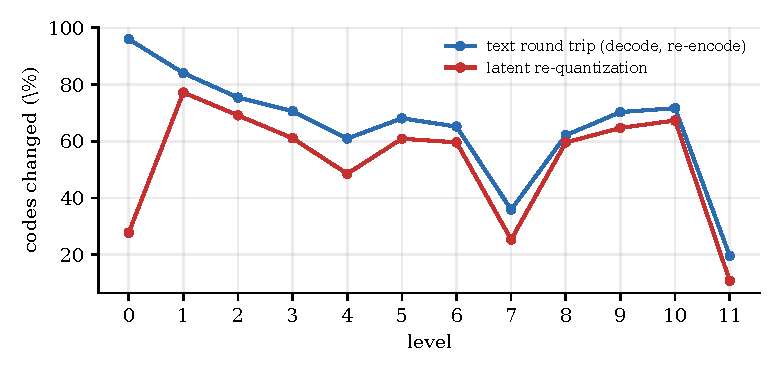
\includegraphics[width=0.66\linewidth]{figs/changed.pdf}
\caption{Share of codes changed per level when the draft's stack is replaced by the tokenizer's stack for the same text (blue) or by the re-quantized latent (red), TinyStories, 768 samples.}
\label{fig:changed}
\end{figure}}{}

\subsection{Is it a temperature schedule? Exact twins and human text}
\label{sec:twins}

Because attention is block-diagonal, level $j$ sees only $\hat z_{j-1}$, so resampling levels $\geq k$ from the draft's own coarse codes is distributed exactly like the draft. Every refinement recipe therefore has an exact 11-pass twin: the same per-level temperatures, no round trip. Table~\ref{tab:twins} compares recipes with their twins on held-out seeds 4--6, together with a temperature curve from $\tau{=}0.6$ to $1.3$ measured on the same seeds.

\begin{table}[!htb]
\centering
\small
\setlength{\tabcolsep}{4pt}
\begin{tabular}{lrrrrr}
\toprule
Sampler & NFE & Gen.\ PPL $\downarrow$ & dist-3 $\uparrow$ & xs-4 $\downarrow$ & vs.\ $\tau$ frontier \\
\midrule
\tabinput{tables/twins.tex}
\bottomrule
\end{tabular}
\caption{Refinement recipes and their exact 11-pass twins (same per-level temperatures, no round trip), TinyStories held-out seeds 4--6. ``$\tau_{\geq k}$'' sets the temperature of levels $\geq k$; parts apply in order. Human rows apply the rounds to 768 real validation openings instead of a draft.}
\label{tab:twins}
\end{table}

At the released temperature the twin of $\RT{6}$ is the released sampler itself, and refinement accounts for the whole $-14.5\%$. With hot coarse and cool fine levels the picture is more nuanced: the per-level schedule alone already lies well below the global-temperature curve ($-21.0\%$ for the twin of the best recipe, $-11.3\%$ for the twin of the $\tau{=}1.2$ recipe), and refinement adds 4--10 points on top ($-25.2\%$, $-21.4\%$). We therefore report the hot-draft samplers as ``schedule plus round trip'' and attribute to refinement only its increment. On LM1B large the twin of the hot-draft sampler is far worse at a similar entropy (90.27 vs.\ 63.37, entropy 4.361 vs.\ 4.368).

Applied to real human text instead of a draft, refinement does not lower Gen.\ PPL below that of the human text: one round raises it from 8.51 to 9.39 with distinct-3 and cross-sample overlap essentially unchanged (0.772 vs.\ 0.775, 0.141 vs.\ 0.139), and further rounds raise it more. A sharpening operator would push human text to lower perplexity and lower diversity; round-trip refinement instead moves the generator's drafts towards the text it was trained on and leaves real text close to where it is, apart from the generator's own realisation errors.

\subsection{Does it transfer to images?}
\label{sec:var}

Next-scale image models face the same structural situation: VAR \citep{tian2024var} samples a stack of multiscale residual codes and decodes it with a VQ-VAE. We applied the round trip to the released VAR-d16 ImageNet-$256$ model with its FID sampling settings, copying its sampler verbatim and only forcing the coarse scales: decode the draft to an 8-bit image, re-encode it with VAR's own VQ-VAE, keep scales $<k$ and regenerate the rest (Table~\ref{tab:var}; 10 images per class, FID-10k against the ADM reference images with Inception features from \texttt{pytorch-fid}). Forcing every scale to the draft's own codes reproduces all 2{,}000 test drafts exactly. The phenomenon carries over: the image round trip changes 29--92\% of the codes at the first nine scales. The benefit does not: the best restart moves FID from 9.13 to 8.92, while resampling without re-encoding, which draws from the released distribution, already moves it to 9.22, so differences of 0.1--0.2 are within noise, and restarting from coarser scales is worse. Unlike text, the pixel round trip is lossy, and VAR conditions every scale on all earlier scales rather than on the latest reconstruction only; either may explain why canonical coarse codes do not help there. We did not run the 50k-sample confirmation.

\begin{table}[!htb]
\centering
\small
\begin{tabular}{lrr}
\toprule
Sampler (VAR-d16, ImageNet 256) & FID-10k $\downarrow$ & codes changed by the round trip \\
\midrule
\tabinput{tables/var.tex}
\bottomrule
\end{tabular}
\caption{Round-trip refinement on an image next-scale model. The round trip goes through an 8-bit image. Code changes are per scale, over the first nine of ten scales.}
\label{tab:var}
\end{table}

\section{What did not work}
\label{sec:negative}

Before finding round-trip refinement we tried six training-side ideas on the TinyStories checkpoint, two of which the NCM paper names as future work. All fine-tunes continue the released generator with AdamW (0.9, 0.95), weight decay 0.1 and gradient clipping 1, as in the paper, but with batch 64--128 instead of 2{,}048 for budget reasons. Table~\ref{tab:negative} summarises them; numbers are GPT-2 Large Gen.\ PPL at full depth unless stated.

\begin{table}[!htb]
\centering
\small
\begin{tabular}{p{0.27\linewidth}p{0.66\linewidth}}
\toprule
Idea & Outcome \\
\midrule
Early exit (adaptive depth) & No plateau to exit into: the last pass alone takes GPT-2 small Gen.\ PPL from 37 to 20.5; the best per-sample stopping rule saves 0.7 passes for $+3\%$. \\
Level skipping at inference & One skipped middle level $+6$--$11\%$, three $+34\%$, five $4.9$--$7\times$, although the tokenizer still reconstructs 98--99\% of tokens from every other level. \\
Level-dropout fine-tuning & With the paper's conditioning corruption, no gain at 8--10 passes; wins only at 6 passes (54.6 vs.\ 79.7), still $3.4\times$ worse than full depth. Without corruption, any fine-tune collapses to 36--40 (exposure bias). \\
Joint tokenizer + generator & Tie: 16.83 (with a coupling loss) vs.\ 16.85 for the generator-only control; reconstruction stays 99.98\%. \\
Own-error corruption & Replacing uniform corruption by the model's own sampled guesses hurts, dose-dependently: 21.8 (half) and 40.2 (all) vs.\ 16.85. \\
Distilling refinement & Training on 50\% refined stories matches the released 16.15 at 11 passes, but at the diversity of $\tau{=}0.8$ (Table~\ref{tab:distill}). \\
\bottomrule
\end{tabular}
\caption{Training-side ideas that did not beat the released sampler.}
\label{tab:negative}
\end{table}

\begin{table}[!htb]
\centering
\small
\begin{tabular}{lrrrr}
\toprule
Generator (11 passes, $\tau{=}1$) & batch & Gen.\ PPL $\downarrow$ & dist-3 $\uparrow$ & xs-4 $\downarrow$ \\
\midrule
\tabinput{tables/distill.tex}
\bottomrule
\end{tabular}
\caption{Distilling round-trip refinement into the generator: 1{,}500 fine-tuning steps on half real stories and half $\RT{5}{\times}2$-refined stories, against a control on real stories only; ``soup'' averages the fine-tune with the released weights \citep{wortsman2021wiseft}. The distilled model ties the released Gen.\ PPL only because it is less diverse: the released sampler at the same distinct-3 ($\tau{=}0.8$) scores 13.34.}
\label{tab:distill}
\end{table}

The distillation result deserves a comment, because without diversity metrics it looks like a near-win: against its own control the distilled model is 3.8\% better on every seed, and fine-tuning drift (the control is 3.9\% worse than the released model) seems to be the only obstacle. Corpus diversity tells a different story. Sequence-level distillation \citep{kim2016seqkd} transferred the refined sampler's lower diversity (distinct-3 0.719 vs.\ 0.749) but not its fluency at that diversity: at matched distinct-3 the distilled model is about 21\% worse than simply lowering the released model's temperature. A larger batch would reduce the drift but not this gap. The common thread of Table~\ref{tab:negative} is that, at this scale, inference-time changes to the released model were far cheaper and more effective than any fine-tune we could afford.

\section{Related work}
\label{sec:related}

\paragraph{Coarse-to-fine and residual-code generation.} NCM \citep{kumbong2026ncm} brings next-scale prediction \citep{tian2024var,kumbong2025hmar} and residual quantization \citep{lee2022rqvae,borsos2023soundstorm} to text. Infinity's bitwise self-correction \citep{han2024infinity} re-quantizes \emph{training} targets after flipping input bits so that later scales learn to fix earlier errors; our method instead re-quantizes \emph{at inference}, needs no retraining, and goes through the decoded tokens.

\paragraph{Re-quantize and regenerate.} The closest prior method is scale-travel in DiverseVAR \citep{park2025diversevar}: re-quantize the accumulated image latent, rewind to a coarser scale and regenerate, used there to restore quality after diversity-boosting perturbations; no base-sampler result is reported. Round-trip refinement differs in going through the discrete output (decode, then re-encode) rather than re-quantizing the latent, in targeting text, and in being evaluated as a base sampler with frontier controls; LatentRQ$_k$ (Section~\ref{sec:why}) is the direct comparison; on NCM it recovers about half of the matched-diversity gain of the text round trip. SDEdit \citep{meng2021sdedit} similarly re-noises an output and denoises it again with a diffusion model, and Restart sampling \citep{xu2023restart} alternates forward noising and backward sampling to correct accumulated errors, the closest mechanism in continuous diffusion. TTS-VAR \citep{chen2025ttsvar} spends test-time compute on scale-wise image generation through selection.

\paragraph{Iterative refinement and self-correction.} Mask-Predict \citep{ghazvininejad2019maskpredict}, MaskGIT \citep{chang2022maskgit}, Token-Critic \citep{lezama2022tokencritic} and ReMDM remasking \citep{wang2025remdm} revise parallel predictions by re-masking and re-predicting tokens; Self-Refine \citep{madaan2023selfrefine} has large LMs critique and rewrite their own outputs. In NCM, codes within a level are conditionally independent given the coarser levels, so re-masking within a level does not apply; the round trip changes the \emph{conditioning} instead.

\paragraph{Exposure bias.} Training on model outputs \citep{bengio2015scheduled,savinov2021sundae} and student-forcing for scale-wise image models \citep{zhou2025sar} address the train--test gap in training; our own-error corruption experiment is in this family and did not help in fine-tuning. Joint or post-training of tokenizers \citep{wang2024larp,leng2025repae,qiu2025tokpost} helps in vision; for NCM text at our scale it tied.

\paragraph{Evaluation.} Gen.\ PPL can be lowered by reducing diversity or by low-precision sampling \citep{zheng2024maskedsecret,pynadath2026frontiers,franca2026hacking}; we therefore report temperature frontiers and corpus diversity alongside it.

\section{Limitations}

Our evaluation relies on Gen.\ PPL under GPT-2 Large, simple diversity statistics, MAUVE and a single 7B LLM judge with a strong position bias that we average out; we did not run a human evaluation, and at equal Gen.\ PPL the judge does not distinguish refinement from a lower temperature. All models are around 100M parameters with 128-token sequences; the OpenWebText checkpoint, the only released model of long general text, was not yet available on the hub when we ran these experiments. Refinement costs 1.3--2.6$\times$ the generator passes and 1.5--3.3$\times$ the generator FLOPs. It fails when the tokenizer round trip is lossy (WMT14), and it does not transfer to the image model we tried (VAR-d16, FID-10k only). Our reproduction of the released TinyStories sampler is 5\% above the paper's number, and all relative claims are against our reproduction. Restart levels and hot-draft temperatures were chosen on the same three seeds we report, from small grids. Fine-tuning baselines were limited to batch 64--128, so the training-side negative results may not hold at the paper's batch size, with the exception of the diversity argument against distillation.

\section{Conclusion}

NCM's coarse-to-fine sampler produces code stacks that its own tokenizer would never produce for the same text. Passing the draft through the tokenizer and regenerating the fine levels repairs this, with no training and a few lines of code, and lowers generative perplexity by 17--31\% on TinyStories and 22--29\% on LM1B while keeping diversity, 10--14\% beyond what temperature can buy and 15--22\% when paired with a hotter draft. The ablations locate the gain in the re-encoding itself: resampling without it does nothing, and re-quantizing the latent instead of the text gives about half. The results hold on held-out seeds and do not shrink with model size; exact temperature twins and real human text show that the gain is neither a temperature schedule nor a sharpener; an LLM judge prefers refined stories; MAUVE moves closer to human text; and on Sudoku the gain is limited to the hardest puzzles, while verifier-guided search is better served by plain resampling. The method needs a lossless tokenizer round trip, and it trades extra passes for quality, so it complements rather than replaces NCM's main appeal of speed. Training-time alternatives that we could afford, including distilling the refined sampler, did not help.

\paragraph{Acknowledgements.} We thank the NCM authors for releasing checkpoints, data and evaluation code, without which none of this would have been possible. This work was carried out independently of any King's College London course. Code and experiments were developed with the assistance of an AI coding assistant (Claude); the author is responsible for all content.

\bibliographystyle{plainnat}
\bibliography{refs}

\appendix

\section{Implementation}
\label{app:impl}

Refinement reuses the released \texttt{NextConceptTransformer.generate}. The only change is a wrapper around its per-level sampling function:

\begin{verbatim}
_orig = net._sample_level
def _sample_with_force(logits, temperature, top_k, top_p):
    level = state["calls"] + 1 - state["offset"]   # level-0 queries counted by offset
    state["calls"] += 1
    if state["codes"] is not None and 1 <= level < state["upto"]:
        return state["codes"][level]               # re-encoded codes for levels < k
    return _orig(logits, temperature, top_k, top_p)
net._sample_level = _sample_with_force

draft = generate(l0)                                # authors' sampler, unchanged
codes = split_levels(tokenizer.vqvae.encode(draft)) # re-encode the decoded tokens
refined = generate(codes[0], forced=codes, upto=k)  # regenerate levels k..K-1
\end{verbatim}

All scripts, run logs and per-seed results are in the accompanying repository.

\section{Samples}
\label{app:samples}

TinyStories, seed 1, sample 4 (same draft for all rows; differences from the draft in bold).

\begin{description}\small
\item[Draft (released sampler).] One day, a little cat named Amy went to a big room to play. In the room, there were many toys \textbf{fun There} were games, and Amy felt happy. She looked and saw a cat. The cat was happy too. The cat tried to catch Amy, but she did not know how. The cat tried to jump high \textbf{to to} reach the cat. Amy felt sad and missed the sad cat. \dots
\item[$\RT{6}$.] One day, a little cat named Amy went to a big room to play. In the room, there were many toys\textbf{. There} were games, and Amy felt happy. She looked and saw a cat. The cat was happy too. The cat tried to catch Amy, but she did not know how. The cat tried to jump \textbf{up high to} reach the cat. Amy felt sad and missed the sad cat. \dots
\item[$\RT{3}{+}\RT{6}{+}\RT{9}$.] One day, a little girl named Amy went to the gym to play. In the gym, there were many kids laughing and playing games. Amy was very happy sound. She looked around and saw a furry cat. The cat was very sad. Amy wanted to help the cat, but she did not know how. She tried to jump high, but she fell down too. \dots
\end{description}

A restart at level 6 keeps the story and repairs local errors; a restart at level 3 re-plans the content (``cat named Amy'' becomes ``girl named Amy'') and, as Table~\ref{tab:ts} shows, trades a little diversity for the largest fluency gain.

\end{document}
